%%%%%%%%%%%%%%%%%%%%%%%%%%%%%%%%%%%%%%%%%%%%%%%%%%%%%%%%%%%%%%%%%%%%
%% I, the copyright holder of this work, release this work into the
%% public domain. This applies worldwide. In some countries this may
%% not be legally possible; if so: I grant anyone the right to use
%% this work for any purpose, without any conditions, unless such
%% conditions are required by law.
%%%%%%%%%%%%%%%%%%%%%%%%%%%%%%%%%%%%%%%%%%%%%%%%%%%%%%%%%%%%%%%%%%%%

\documentclass[
  digital, %% This option enables the default options for the
           %% digital version of a document. Replace with `printed`
           %% to enable the default options for the printed version
           %% of a document.
  table,   %% Causes the coloring of tables. Replace with `notable`
           %% to restore plain tables.
  nolof,     %% Prints the List of Figures. Replace with `nolof` to
           %% hide the List of Figures.
  nolot,     %% Prints the List of Tables. Replace with `nolot` to
           %% hide the List of Tables.
  %% More options are listed in the user guide at
  %% <http://mirrors.ctan.org/macros/latex/contrib/fithesis/guide/mu/fi.pdf>.
]{fithesis3}
%% The following section sets up the locales used in the thesis.
\usepackage[resetfonts]{cmap} %% We need to load the T2A font encoding
\usepackage[T1,T2A]{fontenc}  %% to use the Cyrillic fonts with Russian texts.
\usepackage[
  main=english, %% By using `czech` or `slovak` as the main locale
                %% instead of `english`, you can typeset the thesis
                %% in either Czech or Slovak, respectively.
  german, russian, czech, slovak %% The additional keys allow
]{babel}        %% foreign texts to be typeset as follows:
%%
%%   \begin{otherlanguage}{german}  ... \end{otherlanguage}
%%   \begin{otherlanguage}{russian} ... \end{otherlanguage}
%%   \begin{otherlanguage}{czech}   ... \end{otherlanguage}
%%   \begin{otherlanguage}{slovak}  ... \end{otherlanguage}
%%
%% For non-Latin scripts, it may be necessary to load additional
%% fonts:
\usepackage{paratype}
\def\textrussian#1{{\usefont{T2A}{PTSerif-TLF}{m}{rm}#1}}
%%
%% The following section sets up the metadata of the thesis.
\thesissetup{
    date          = 2017/01/04,
    university    = mu,
    faculty       = fi,
    type          = mgr,
    author        = Bc. David Kouřil,
    gender        = m,
    advisor       = {RNDr. Barbora Kozlíková, Ph.D.},
    title         = {Maya2CellVIEW: Integrated Tool for Creating Large and Complex Molecular Scenes},
    TeXtitle      = {Maya2CellVIEW: Integrated Tool for Creating Large and Complex Molecular Scenes},
    keywords      = {molecular visualization, illustration, Maya, Unity},
    TeXkeywords   = {molecular visualization, illustration, Maya, Unity},
    bib           = example.bib,
}
\thesislong{abstract}{
  Scientific illustrators communicate the cutting edge of research through their illustrations. There are numerous software tools that assist them with this job. Often they use professional modeling and animation 3D programs which are primarily used in games and movies industry. Because of that however these tools are not suitable for scientific illustration out of the box. There have been attempts to address this issue which brought tremendous results.

  This work focuses on visualization of structures and processes in biology, focusing mostly on the scales of nano- to micrometers. At this scale we often do not gain much by using hyper-realistic rendering style that the professional software aims for. Instead we want to employ more simplified style which helps to communicate the important story without losing much detail or scientific precision.
  
  The aim of this thesis is to push abilities of illustrators working on large scale molecular scenes. This is done by connecting two software packages—Maya and cellVIEW—combining the real-time rendering possibilities of cellVIEW and modeling and animation tools of Maya which results in more effective and efficient workflow.
}
\thesislong{thanks}{
  TODO: thanks
 % Many people are directly or indirectly responsible for this work.
  
  %First, I would like to thank Bara Kozlikova for introducing me to the domain of visualization, serving as a mentor to me and building relationships with TU Wien for years before by which she has enabled me the opportunity to work on this thesis in cooperation with TU Wien.

  %Next, I want to thank Mathieu Le Muzic for being my day-to-day coding supervisor while I was visiting in Vienna. I want to thank Mathieu for being a mentor and a role model for me.

  %I thank Ivan Viola for being my remote supervisor and consultant. Thank you for guiding me through the process of writing this thesis, giving feedback and in general going above and beyond with your help.

  %I thank my parents for working hard on providing for me and my sister and creating homely and supportive environment.
  
  %Last but not least, I want to thank my girlfriend Gabi for being
}
%% The following section sets up the bibliography.
\usepackage{csquotes}
\usepackage[              %% When typesetting the bibliography, the
 backend=biber,          %% `numeric` style will be used for the
%  backend=bibtex,
  style=numeric,          %% entries and the `numeric-comp` style
  citestyle=numeric-comp, %% for the references to the entries. The
  sorting=none,           %% entries will be sorted in cite order.
  sortlocale=auto         %% For more unformation about the available
]{biblatex}               %% `style`s and `citestyles`, see:
%% <http://mirrors.ctan.org/macros/latex/contrib/biblatex/doc/biblatex.pdf>.
\addbibresource{example.bib} %% The bibliograpic database within
                          %% the file `example.bib` will be used.
\usepackage{makeidx}      %% The `makeidx` package contains
\makeindex                %% helper commands for index typesetting.
%% These additional packages are used within the document:
\usepackage{paralist}
\usepackage{amsmath}
\usepackage{amsthm}
\usepackage{amsfonts}
\usepackage{url}
\usepackage{menukeys}
\begin{document}
\chapter{Introduction}
\label{chap:introduction}
%[\textbf{In what field are we? What are the people in this domain doing?}]
In this day and age, scientists come to new findings every day. Unfortunately, not all of these are ever shown to the general public. There can be several reasons for that. New discovered facts are usually pieces of a bigger picture. Also, all the information might be already there, in several databases, but putting it all together would take significant effort and time.
On top of that, scientists are not usually trained to expose their results to the public eye.

This is the job of scientific illustrator. These people are, first and foremost, experts in their fields but on top of that they have invested significant amount of time on acquiring and perfecting their artistic skills. They use these skills to visualize the science in their domain with easily understandable images, animations or other forms of media. %if somebody asks - ex. arthur olson 3d prints and sculptures
\begin{figure}
  \centering
  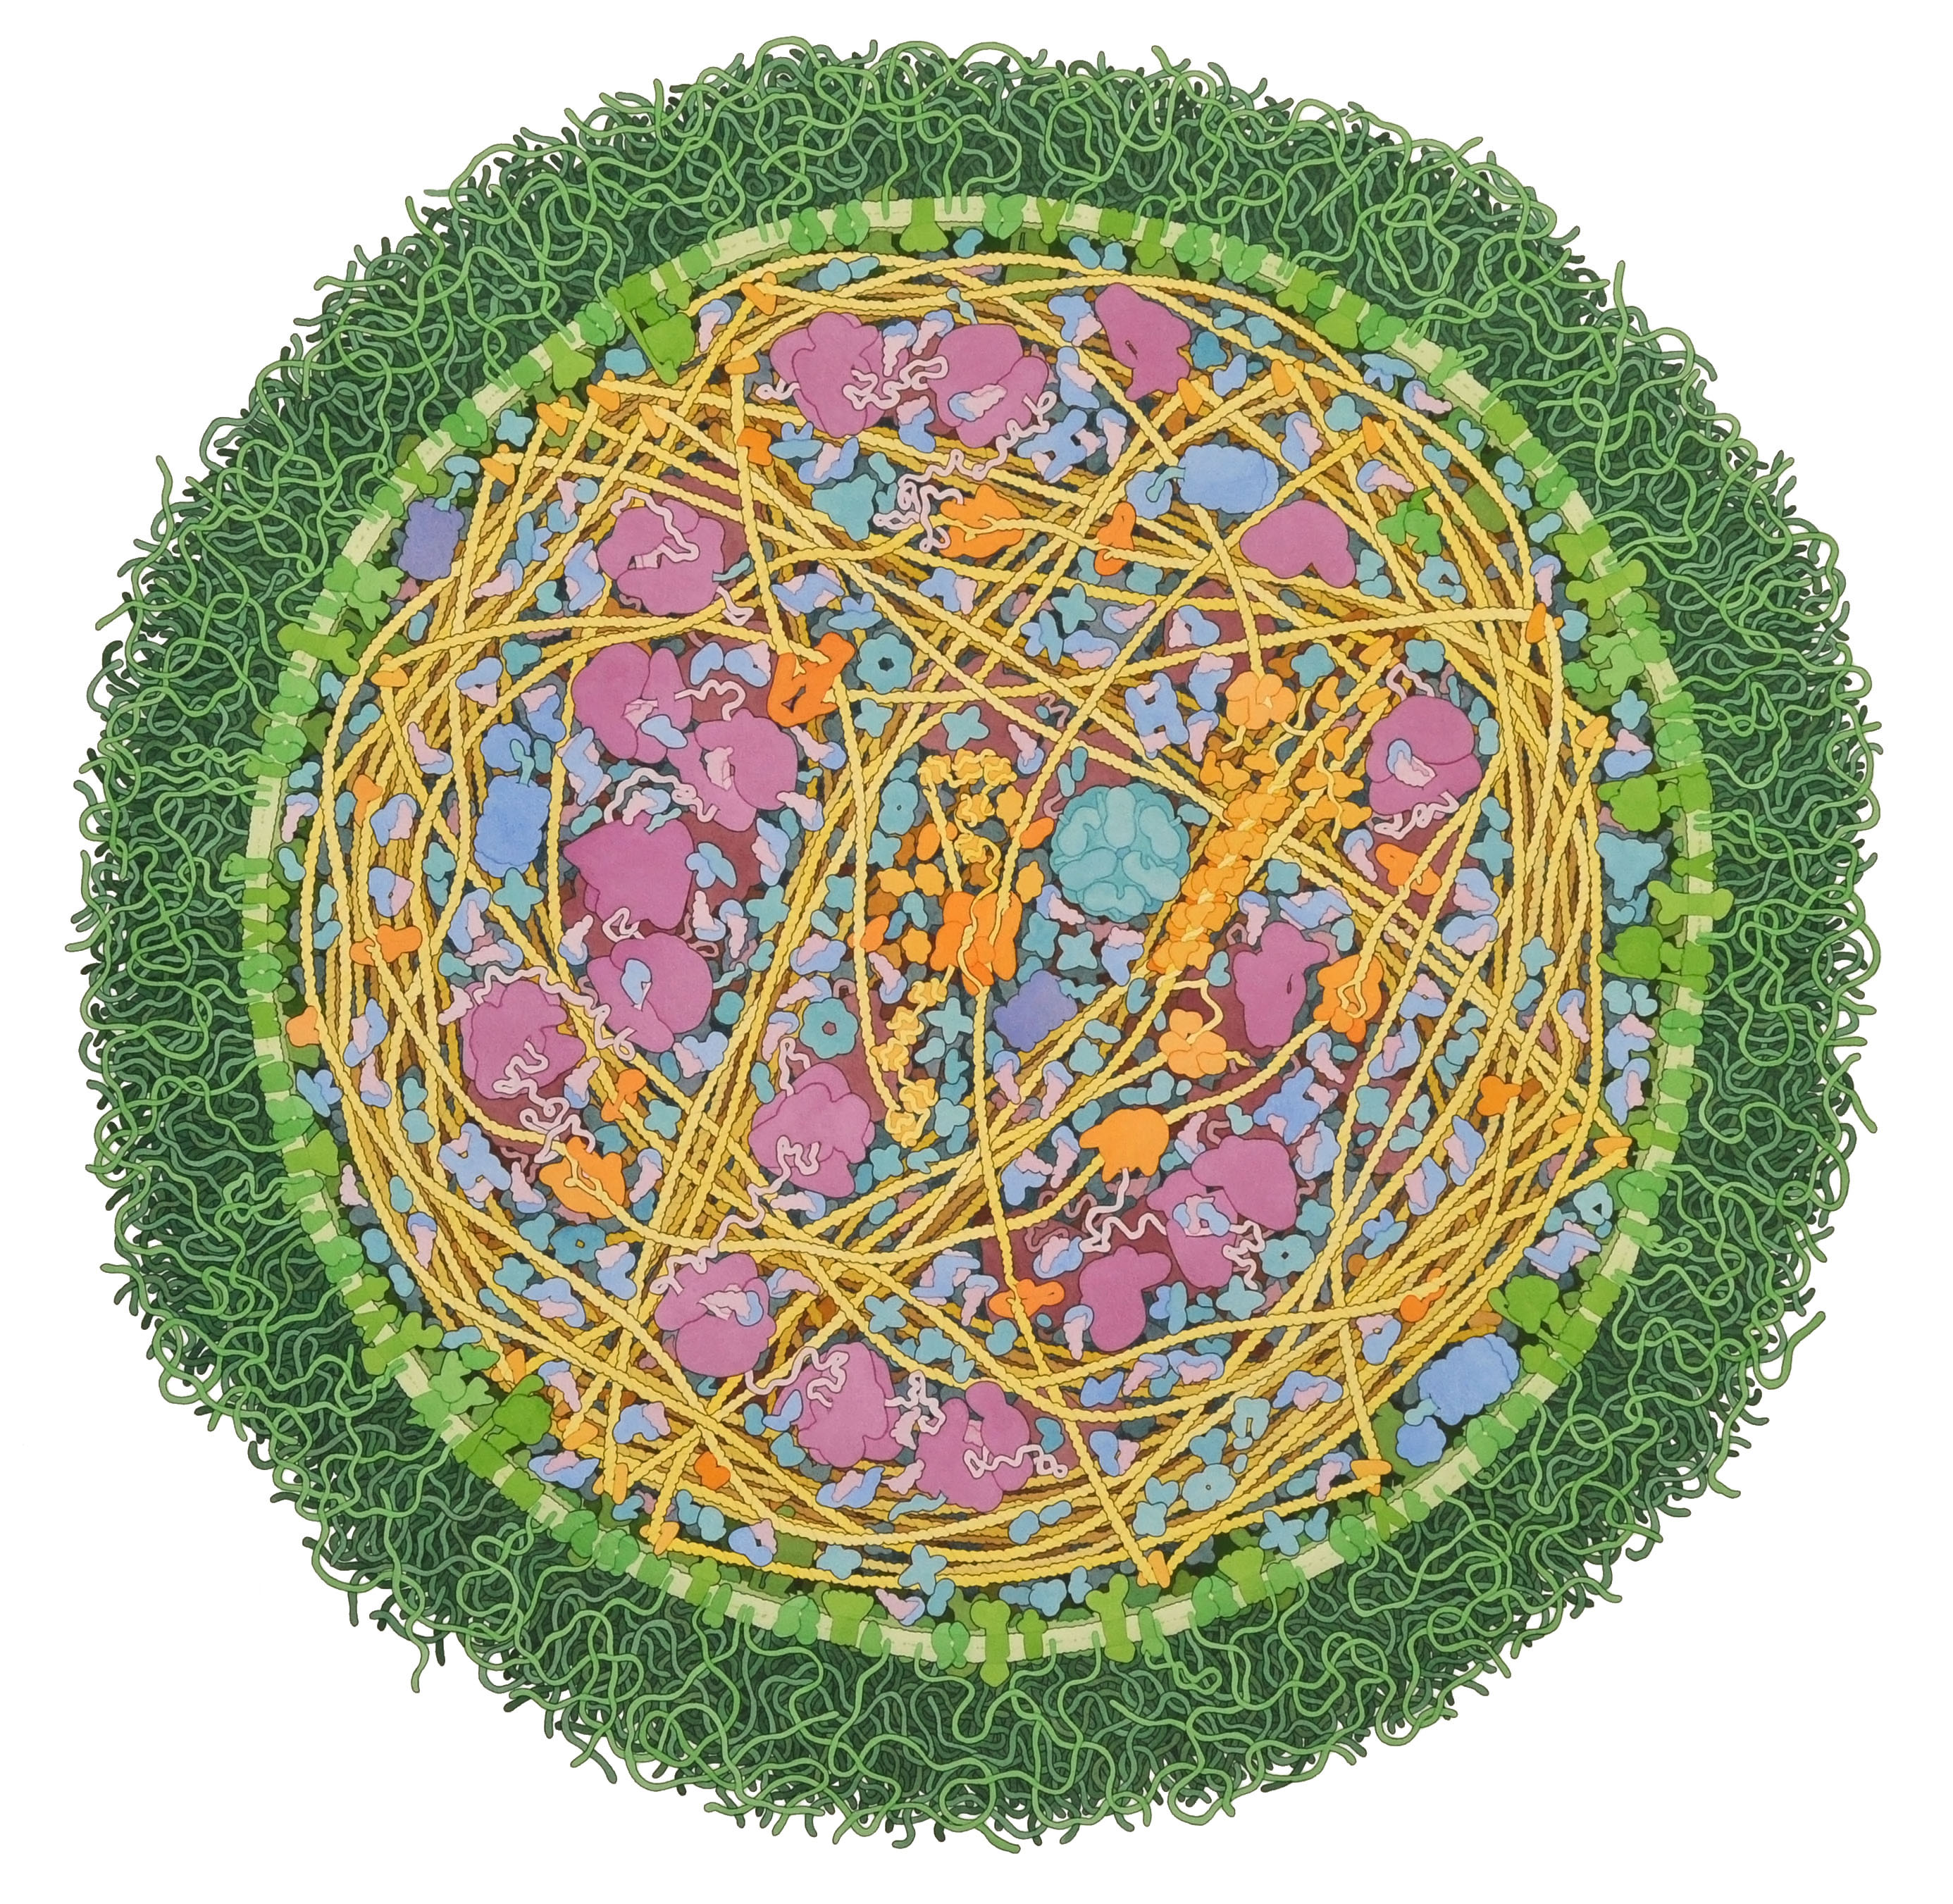
\includegraphics[scale=0.4]{images/goodsell-mycoplasma.jpg}
  \caption{David Goodsell's illustration of}
  \label{fig:goodsell-mycoplasma}
\end{figure}
% TODO: say that we are in domain of biological/molecular visualization
This thesis focuses on visualization of structure and function of objects in cell and molecular biology. To show examples of such visualizations we can point to works of Drew Berry \cite{DrewBerryMovies}, Graham Johnson \cite{GrahamCellVideo} or Janet Iwasa \cite{iwasa2010animating}.

% TODO: [\textbf{why are illustrations/animations useful: what art was talking about and also janet in molecular flipbook video}]
The importance of such work is not only in bringing the science to the laymen. Humans are visual beings and by seeing something we can understand certain concepts more deeply or differently. And this applies to other scientists as well. In practice this means that such artworks can serve as a discussion starters. New ideas, hypothesis and experiments might emerge just by seeing concepts differently or as a compilation of information into one cohesive artwork.

Scientific illustrators have to balance both the correctness and artistic form of their outputs. Where conventional artist can use visuals to suppress or pick up his message however he wants, illustrator is limited by the boundaries of scientific correctness. In the past, simplifications in such works have often been criticised by the experts as misleading.

There are many ways how scientific illustrators can do their job. Historically, illustrations have been done by hand with traditional drawing and painting methods. Even today, some illustrators still prefer this way of working. It is however a very timely process, as individual illustration can take months to make. Probably the most well known and accomplished person in this is David Goodsell\footnote{
  David Goodsell's web page: \url{http://mgl.scripps.edu/people/goodsell/}
} whose work is shown in Figure \ref{fig:goodsell-mycoplasma}. Goodsell has developed a style of abstracting details while preserving the general shapes. However, this is a very timely process, as individual illustration can take months to make\cite{DavidGoodsellVideo}. If we consider the speed at which science is moving forward nowadays what could end up happening is that before an illustration is finished a new finding emerges, rendering the illustration effectively obsolete. This is of course undesirable and we need to look for ways how to accelerate, or even partially automate, this process.

% [\textbf{Can we use computer graphics for this?}]
With the increasing popularity of computer generated imagery, it has naturally been adopted by scientific illustrators as well. Tools have become more accessible and easier to use over the years. Today, software solutions like Maya, Cinema4D or 3Ds Max have become industry standards for any task that revolves around modeling 3D geometry and rendering it. Game and movie industry are the leading industries that push computer graphics software creators forwards and provides most of the revenue for them. This means that these tools, no matter how versatile they try to be, are being skewed towards the use cases in movies and games. That means that people who want to create scientific content might struggle to use the tools sometimes. Still, people have been able to create amazing images and movies showing people phenomena from all kind of science disciplines.

% before it was hard to make illustrations, now it's even harder because we want to do animations
With traditional methods it was timely to create just a static illustrations. This process can be sped up by using modern tools with the help of computers. But the bar has been raised by the need of animated content and movies. Now this is what can take months to prepare. Using professional 3D tools certainly helps. For example, instead of frame-by-frame animation, physics simulations can be used to create animations which are (at least to a certain extent) physically correct. The problem still persisting is that vendors do not design their products with a use in scientific illustration in mind. It would actually be impossible to do so when we take into account how much different uses we would like to employ this software. But we still need a way how to import scientific data into the program and work with them.

To do that, people have learned to customize this software\cite{GrahamGaelInterview}. Commercial 3D authoring software is by convention highly customizable via scripting and/or APIs. This allowed illustrators and animators to extend the software by implementing functionality that they need. For example, one task that commercial toolsets do not solve is loading scientific data and structures as models. Some of these have been released to public (as we will see in chapter \ref{chap:star}) but most of the scripts are being developed and used only by the original author.

% [\textbf{what are the alternatives to what people are using already?}]
From a completely different section of the field of molecular visualization, there are domain-specific tools. There is an active research in the domain of visualization, with many conferences every year and hundreds of research papers in this field coming out. Usually, as a byproduct, these papers generate software that showcases the proposed visualization technique or pipeline. Some of these have been turned into full featured visualization packages and thus provide a way how to illustrate something in a new way. While these programs might hugely benefit scientific illustrators, it is not always the case that they get used. Usually illustrators are simply used to a certain pipeline and incorporating a new software into this pipeline does not seems very beneficial to them. Another problem is that because these programs are developed for a certain use cases (showcasing the point of the paper) they might not be easily applicable to more than one purpose.

% [\textbf{``mission statement'' of the thesis}]
%In this thesis, we made an effort to solve these problems. Our domain of choice is molecular visualization.

%In this domain we try to visualize living (?) organisms on the smallest possible scale. With this approach, the computer memory and performance requirements are very challenging even for todays available hardware. Still, people have been able to visualize for example model of HIV in blood plasma in it's full detail down do individual atoms of each protein. This however, is achieved by using a very customized rendering method and a custom data format. In 3D graphics, data are usually represented as meshes consisting of triangles (which in turn are made of vertices). If we wanted to represent each atom as a sphere, we would need at least <number> of vertices for one atom and that's only for the roughest level-of-detail. With such representation, a one whole protein could use up to X bytes of memory which already takes up most of the video cards' memory. Thus this representation is not suitable for this task. Instead, various other techniques have been developed for rendering on molecular data.

%That being said, these techniques are not usually taken into account when 3D authoring software is developed. As was mentioned, the primary users of these software are video games and movies industry, where mesh representation is the one used. That implies that people that use these programs don't have access to the cutting edge technology of rendering, visualization and illustration of molecular data and there is room for us to improve this situation.

The main motivation for this project comes from talks between researchers of Visualization Group at TU Wien and animator Drew Berry. Rendering capabilities of cellVIEW (see Chapter \ref{chap:star}) have been shown to Berry and he has expressed his interest in the style of rendering that developers of cellVIEW have been able to create. Since Drew Berry has been using Maya software for years to create his animated movies, we have decided to investigate if, and how, it would be possible for him to use cellVIEW for his creations in combination with Maya.

In next chapter, we will describe the state-of-the-art programs and tools that are used for molecular visualization today and we will mainly focus on showing the gaps in intercompatibility of the available programs. Then, in Chapter \ref{chap:method}, we will propose a method of how one particular problem could be solved. Chapter \ref{chap:implementation} is dedicated to in-depth description of our implementation. Chapter \ref{chap:demonstration} will demonstrate use cases of implemented method. Finally, in Chapter \ref{chap:discussion}, we discuss the outcome of the whole project and contemplate how it could be extended in the future.

\chapter{State of the Art}
\label{chap:star}
%I think the sections could be: 3D Modeling Software (Maya, C4D), Niche (Specific) Tools (cellVIEW, ...), Data Generation (cellPack)
%Popsat: Molecular Flipbook, Molecular workbench, molecular maya, mcell, cellblender, pymol, VMD, ePMV(scripps)
Several approaches can be taken when creating an illustration, animation or interactive experience that has some basis in science. We will show tools that help with this process, describing its primary use, discuss its implementation and how this tool is or could be used. Listed solutions are the ones which we believe are or were pivotal or at least present ideas which we think are beneficial to this field.

First however, we will talk about the character of data that we are working with in the field of molecular visualization.

\section{Molecular Data}
All matter consists of \textbf{atoms} which are grouped in \textbf{molecules}. Atoms in turn contain protons, electron and neutrons which have their own internal structure. This is a level which is out of the scope of what is relevant to this thesis. Individual atoms are the smallest elements that we will consider.

\textbf{Biomolecules} is a term describing any molecule that takes part in some process in living organisms. \textbf{Macromolecules} are molecules that are very large, containing typically several thousands of atoms or more. We will not be dealing with chemical properties of molecules and therefore details like what forces hold which elements together are omitted. We are mostly interested in the structure of such objects-what they look like.

\textbf{Proteins} are macromolecules that are formed by a process called protein synthesis. During this process, part of DNA is transcribed into messenger RNA which is then turned into chain of amino acids that fold into a protein.

\textbf{Lipids} are hydrophobic molecules that typically serve as a building blocks of lipid membranes. Lipid membranes' function is to separate different compartments in a cell.

% TODO: acquisition
Different techniques are used to acquire molecular data. The three most widely used are X-ray crystallography, nuclear magnetic resonance spectroscopy (NMR) and cryo-electron microscopy (cryo-EM). Each of these techniques has their benefits and downsides. For example, using NMR, only structures of limited size can be resolved. On the other hand, using cryo-electron microscopy can be used to resolve large structure but only in low resolution.

% TODO: pdb
RCSB Protein Data Bank is a database where the information about structure of large biological molecules resolved using these techniques is stored. Each molecule is identified by a PDB ID—alphanumeric code that is 4 characters long. Data can be exported and downloaded in several formats, most notably PDB file format with extension .pdb. For us, the most relevant data that can be acquired from this file is the list of atoms with their XYZ coordinates.

% TODO: cellPACK
Between the molecular (observable with methods like NMR and X-ray crystallography) and cellular scale (observable with microscopy), there is an intermediate scale (mesoscale, 10-100nm). In general, there are no good method available to observe objects in mesoscale in atomic detail. Because of that models on this level must be compiled computationally by using information from multiple sources. cellPACK\cite{cellPACK} is a software that does exactly that. With cellPACK we can assemble models of an intermediate scale by employing packing algorithms. A recipe serves as an input for this algorithm. A recipe is a compilation of data from light and electron microscopy, x-ray crystalography, NMR spectroscopy and other biochemical data. The process then has two steps: gathering of the data to compile a recipe and then assembling a virtual model from this recipe. cellPACK has been developed at Scripps institute and is a biological version of a more general software called autoPACK. Both of these are implemented in Python and open-sourced.

%\section{Commercial 3D Software}
\section{Professional 3D Software}
% [\textbf{Commercial 3D software is absolutely dominating}]
Using a professional 3D modeling and animation software can help scientists to communicate their ideas. These programs have been designed to provide means for people that need to create three dimensional models of any kind. And in the past several years, more and more scientists do employ professional 3D solutions into their pipeline for various purposes.

Unfortunately, these programs usually come with a very steep learning curve. Mastering this tool, or even just getting on level of proficiency that is enough to produce any meaningful work, is not an easy task and takes between several months to years. This is not something a lot of researchers are willing, or even able, to sacrifice. The good news is that there is usually a number of learning materials available on the Internet, both supplied by the vendor of the software and third parties.

Another problem with software meant to general 3D editing is that these tools are not designed with molecular visualizations in mind. This is problematic because of the fact that scientific illustrators mostly want to work from accurate data. Mentioned software is primarily designed to be used by workers in entertainment industry. Thus there is missing any framework which would enable to import scientifically accurate data in the basic program installation.

There is number of options to choose from currently available products. Most widely used are Autodesk Maya and Cinema 4D although other programs, like open-sourced Blender or a relatively young MODO\cite{MODOscientificIll}, have been successfully used in various projects.

Despise the mentioned drawbacks, professional 3D software is being widely adopted as a solid base of workflow of scientific illustrators and animators. Once illustrators overcome the initial learning period, general 3D software becomes a powerful tool in their toolset. 

% TODO: what are the difference, are some better than others in some regards?

% [\textbf{things that are nice to have from these programs - easy manipulation with objects, scene graph to organize the scene, tools for animation, semi-automatic object positioning (random, particles)}]
\subsection{Key Features}
Disregarding the differences between all the 3D software of this kind, there are features that are more or less contained in all of them and over the years have become must-have features that tremendously help with navigating and editing of 3D scene.

First, objects in scenes are organized into some variation of \textit{scene hierarchy} or \textit{scene tree}. This allows users to organize their objects and establish parent-child relationships between these objects.

Second, navigation in the 3D scene is always designed to be intuitive enough to provide efficient ways how user can position his view. Every named program allows the user to open multiple viewports at the same time where every viewport shows different camera position.

Third, object manipulation—translation, rotation and scale—is solved and made available under shortcut which allows the user to work efficiently. Shortcuts are often instruments each individual artist gets used to and might have a hard time switching to different product.
% TODO: images: scene hierarchy across the programs: maya, c4d, blender?
% TODO: images: object manipulation
% These are the killer features and even though they are present in all of the programs, the illustrators are often used to the way they work or to a certain shortcut which means that it's not trivial for them to switch from one to another (or it is but it takes some time).

\subsection{Rendering}
% TODO: rendering
Important component of any professional 3D program is a renderer. Renderer is a tool which turns the 3D scene into a final image (or series of images in case of an animation). All of the mentioned products come with at least one default, pre-installed, renderer. On top of that, user can install external rendering solutions, either commercial or free-to-use. This installation is most often done via plug-ins.

% TODO: offline rendering algorithms
The process that these rendering solutions use is sometimes referred to as ``off-line'' rendering. The opposite of this would be real-time rendering. The difference is mainly in the amount of time that these two types of rendering take. Off-line rendering has taken physical correctness and/or realistic look as its primary goal while the amount of  time the rendering process takes is given less priority. Actual numbers are dependent on the complexity of the geometry in the scene and the materials and effects used in this scene. But the ranges are from several minutes to hours for casual purposes. On the other hand, real-time rendering aims to generate a picture several times each second. The obvious benefit here being that the scene can change dynamically and is still rendered with a frame-rate that human eye consideres a continuous movement. In past the benchmark of 30 FPS (frames per second) has been considered to be the standard, however these days 60 FPS is starting to be more and more common. For 30 FPS, every frame has to been rendered in under 1/30 s = 16ms. In real-time rendering, rasterization\cite{rasterization-paper} is considered the state-of-the-art approach as it enables us to achieve interactive performance fairly easily. Ray tracing (and it's variants) is the type of algorithm used in off-line rendering\cite{pbr-book}.

Plethora of external off-line renderers exists these days. From the popular commercial ones like OTOY's Octane, Chaosgroup's V-ray, Pixar's RenderMan to open-sourced solutions—LuxRender or Cycles (which is now available in default installation of Blender).

In the same way as with particular modeling software, the choice of the renderer is mostly personal choice of the person using it. Renderers are, too, complex tools  which take some time to truly master. This means that when somebody learns how to use a certain renderer they usually stick to this solution.

\subsection{Plug-ins}
%[\textbf{We have an ``entry point'' which we can exploit to inject our custom functionality}]
It has become a convention that all of the professional 3D authoring packages (like Maya, Cinema4D or even Blender) provide one or more means of how users can program additional functionality themselves. There are two major ways how vendors accomplish this.

First, scripting interface is provided. This means that user can both perform operations and trigger actions by using Graphics User Interface (or GUI) but in addition to that they can do the same (and in most cases even more) by calling particular commands via a command-line-like interface. Obviously the capability of these additional implementation is limited and scripting interface is mostly used to automate tasks which would otherwise take too much time.

Second way is the ability to load plug-ins that use Application Programming Interface, or API, designed by the vendor. API provides classes and functions that can access and alter internal state of the program or the data inside it. This way the user can implement functionality that he or she is missing from the basic program. Thanks to that these 3D authoring programs can be adapted to more specific use cases.

%[\textbf{Tools where people already used this plugin architecture}]
Some of these plug-ins have actually already been implemented to help artists in molecular illustration. The most typical functionality implemented is a way how to load molecular data into the program.

An example of that is Molecular Maya\footnote{Available to download at: \url{http://www.molecularmovies.com/toolkit/}}, which, as the name suggests, extends Maya with the ability to load and manipulate models of macromolecules. These can be loaded either from PDB online database or by loading a pdb file from disk. After the molecule is loaded, user can select how by which representation should it be displayed. One of the functions also creates mesh model out of this molecule. User is able to select in which level of detail this export will be performed. Molecular Maya plug-in is free to use with the option to purchase upgraded version that provides more advanced functionality.

BioBlender provides similar functionality for Blender software. MCell and CellBlender\cite{mcell}, plug-ins also for Blender, focus more on the function of proteins and simulation of these processes.

%Similar plugin exists for Blender modeling program as well. It's name is cellblender
% TODO: bioblender: http://www.bioblender.eu/

%[\textbf{How people normally render - offline}]
%The rendering stage takes place after the scene is modeled. Again, there are more options at hand. 3D packages usually come with a default rendering solution which is for the most part good enough to use. For more demanding artist, external renderers like vray, mental ray, corona or octane. What these renderes have in common is that they are so called ``off-line renderers''. In practice this means that they are using ray tracing (or similar) technique to render the scene with a process that is very much close to how light works in real life. The disadvantage of this approach is that this process take more time. It usually is not possible to achieve real-time rendering (fps at least 25).

\section{Domain-specific tools}
%kinemage (http://kinemage.biochem.duke.edu/), chimera (http://www.cgl.ucsf.edu/chimera/), jmol?
%[\textbf{intro}]
In the field of molecular visualization as a separate research topic, numerous programs exist. They share a some features but they each have their own specialties and are meant to be used for slightly different tasks. We will name a few that have been developed for some time and have matured to a certain extent. Apart from that, other tools exist which are even more specialized. These might be results of a research and they accompany a paper describing the technique. This means that these programs are not that well usable out-of-the-box but rather serve as a demonstration of a certain technique.

%\textbf{Molecular Flipbook}
One of the more user-friendlier and easier to use tools is \textbf{Molecular Flipbook}. It has been developed by a team lead by Janet Iwasa and it consists of two parts - an animation program and a website where creators can share their outputs. Main motivation for this project is to create tool that even scientists without education in animation can use to communicate their ideas through simple molecular animations. They achieve this by building the program around the concept of simplified key-frame animation technique. The website portion of the project is meant to serve as a database of animations explaining various processes. Creators can upload their works and improve works of others. Molecular Flipbook has has been build on top of Blender's game engine functionality.
%[\textbf{TODO:} cons, done on top of a blender game engine, info: http://mikepan.com/flipbook.html]

%\textbf{Molecular Workbench}?

\textbf{PyMol}\cite{PyMOL} is a molecular visualization system aimed to be used by expert users. It is an open-source software product in which the user can view, render, animate and export 3D molecular structures. PyMOL can visualize molecules with several representations—spheres, surface, mesh, lines, sticks, etc. Rendering of high quality images can be done with internal ray caster.

PyMOL focuses on visualization of individual macromolecules, not so much used to create molecular scenes which contain several thousands of these.

\textbf{VMD} (Visual Molecular Dynamics)\cite{HUMP96} serves as a tool for modeling, visualization and analysis. It actually has a long tradition, being first introduced in 1996. Similarly to PyMOL, VMD has been used extensively to make figures and illustrations for covers of textbooks and journals. Its primary purpose lays in molecular modeling—using computer simulations in applicati

\textbf{cellVIEW}\footnote{Additional information and links available at https://www.cg.tuwien.ac.at/research/projects/illvisation/cellview/cellview.php}\cite{cellVIEW_2015} is a tool with the ability to render large biological macromolecular scenes at an interactive frame-rates. It has been designed and implemented with regards to this use case with the use of state-of-the-art rendering techniques. It employs several modern techniques to reduce the amount of processed geometry in macromolecular scenes to provide its users with a real-time performance. As a result cellVIEW can render scenes containing up to several billion atoms with a frame-rate above 60 FPS. cellVIEW has been implemented with Unity game engine. The rendering styles has been inspired by illustration by David Goodsell who has developed a style of abstracting the shape of individual proteins to reduce visual noise of the picture. cellVIEW imitates this approach by incorporating a level-of-details scheme. The farther the protein is from the camera the less amount of its atoms are rendered and the rendered atoms are scaled up. This approach results in a multi-scale visualization—user can zoom in to see individual atoms of a protein instance, or he can zoom out and see the whole dataset with its distinguishable compartments. The biggest dataset that has been visualized using cellVIEW is human immunodeficiency virus (HIV), however performance tests that have been done indicate that larger datasets (e.g. Escherichia coli bacterium) should be possible to render as well.

%\begin{figure}
%  \centering
%  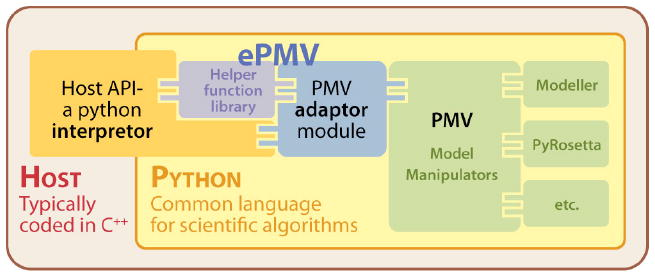
\includegraphics{images/epmv-architecture.jpg}
%  \caption{ePMV architecture}
%  \label{fig:ePMV}
%\end{figure}
\textbf{ePMV}\cite{ePMV} tackles similar problem as we do. The goal is to simplify process of generating figures and animations for scientific purposes taking into account the fact that illustrators have tools that they are familiar with. ePMV is a plug-in which brings molecular visualization toolset into various 3D authoring software, in this context called host. They take advantage of host API which is nowadays commonly exposed to be used by custom Python scripts. By implementing they create an unified environment where the molecular visualization software can run. Thanks to this unified environment, an adaptor, the molecular program can stay the same across all the supported hosts. Only the adaptor needs to be adapted to a new hosts' API. When designed, emphasis has been given to making sure that both native (general 3D modeling) and scientific molecular tools are used in conjunction to their full potential.

Several host programs are already supported—Cinema4D, Blender, Maya and 3ds Max, with plans to extend this list further.

\section{Workflow}
% [\textbf{Define the workflow - how it is now and how we could improve it (fasten it)}]
The actual workflow obviously differs from illustrator to illustrator, different software is used, different plug-ins and most importantly different data and project goals.

It is however important to formalize a little bit how the workflow looks like. Our goal is to connect one of the specific domain tools into a professional software. By doing that, we want to achieve faster and therefore more effective workflow.

We consider the pipeline to be composed of two major steps - modeling and rendering. In the modeling step, all the data, requirements, hypothesis, ideas and stories are compiled into a 3D scene or animation. Artist usually uses software-specific features like particle systems or physics simulations to get there.

The next step is generation of either still image or animated video from the 3D scene/animation. This is equally, maybe even more so, important as the first step. By using certain rendering techniques we can underline concepts which are important to the artwork. The level of detail has to be carefully chosen not to overwhelmed the audience with visual noise. Traditionally, the rendering step has been very computationally intensive. Today with the power of modern GPUs and the increasing availability of such devices, the render times have been reduced dramatically. Still, this represents an obstacle in the workflow of animator. Even just one minute delay can cause distraction.

% yeah it's good to end this with workflow because I can talk here about how things are and what is the problem that we want to solve and in method I can continue with that and it's exactly as we talked with Ivan about the Problem definition
This is the problem that we wanted to solve by using custom state-of-the-art molecular renderer. As was mentioned before, at this domain, hyper-realistic results of modern rendering methods are not that beneficial to us. We instead want to employ more illustrative, simplified rendering styles. That brings us another benefit in that this rendering method is better performing allowing us to render at interactive (real-time) frame-rate. By using our fast renderer, we want to eliminate the time cost of rendering step when using conventional off-line renderers.

\chapter{Method}
\label{chap:method}
%[\textbf{we focus on fastening the workflow by using our renderer}]
As was discussed in Chapter \ref{chap:star}, the majority of artists uses professional (often commercial) 3D software. These programs are very good at modeling and rendering 3D content as a set of meshes—3D objects consisting of triangles. However, for molecular data and scenes, mesh is not the best representation and there exist rendering techniques that perform way better if we use other representation.

%[\textbf{we can take advantage} of the fact that illustrators use illustrative style, simplified and the data is very compact actually so we can provide them the interactive preview]
Another thing we can take advantage of is that illustrations and animation describing structures and function of objects at nanoscale do not often profit from using ultra-realistic rendering. The concept of realistic rendering and light/material interactions do not exist at this scale. They show concepts that are happening at different scales than the stuff that programs are usually made for. Thus they usually want to use more illustrative, simplified, rendering styles.

In our use case, this is even more true because we are dealing with a very dense data sets. We want to simplify what we show to reduce the visual noise in the output image. Various level-of-detail (LOD) schemes exist and they not only help with filtering of the visual noise but also reduce the performance requirements.

Thanks to these simplifications we can render molecular scenes with interactive frame-rates, as has been shown by cellVIEW\cite{cellVIEW_2015}. Unfortunately, these techniques are not implemented in 3D commercial programs which is what the artists usually use. Our goal is to make it so that the artist can use his software of choice to model his scenes but also take advantage of modern rendering. The use is two-fold: real-time rendering can serve as a preview of the scene but also can be used as a final result. The goal of this project was to come up with an idea of how to connect these two programs so that they will work together.

%[\textbf{two options, we choose third}]
Ultimately, we have two programs and we want to use some functionality from the first one and other functionality from the second one. The naive solution would be to implement our desired functionality into the software that is missing it. In our case, that would mean we could either implement the fast and visually appealing rendering into our modeling software, or we could do the opposite and implement the desired modeling tools into our renderer.

The problem with the first approach is that substantial percentage of the 3D software packages that artists are using the most are commercial solutions with closed source code. It is possible to extend them via API that they provide but that is not enough if we want to implement state-of-the-art technique that sometimes requires the latest technology in terms of graphics API etc.

We also do not want to implement desired 3D modeling tools into our specific domain program. This would create development overhead which would not bring much benefit on its own. Besides that, every artist uses different instruments and gratifying all of them would be impossible thing to achieve.

\begin{figure}
  \centering
  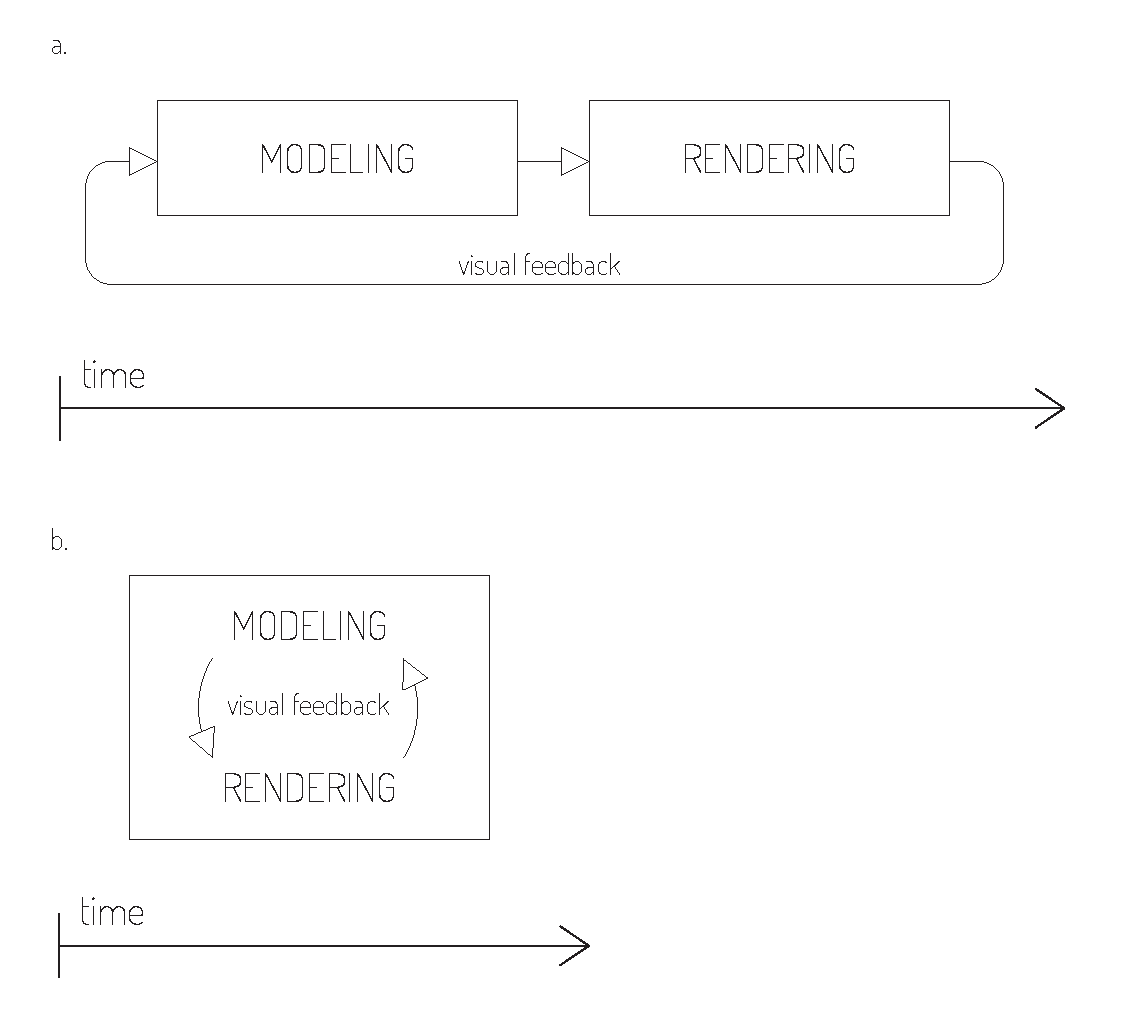
\includegraphics[scale=0.7]{images/workflow-before-after.pdf}
  \caption{Workflow, a. traditional approach with offline rendering, b. our approach with real-time rendering}
  \label{fig:workflow}
\end{figure}

We have chosen to go with another, third, option instead. We do not want to re-implement from scratch something that is already available to use. Instead, we went for a different approach and tried to connect the two parts in a way that would allow us to use both sets of features at the same time. We do this by using both of the programs and establishing a communication channel between them. We use writing and reading from shared memory to accomplish this communication. In our case the communication is one-way. We can model the scene on one side and we want to transfer data describing this scene to have it rendered on the other side. As we will show this can be done in a straight-forward fashion as our scenes can be simplified to the point when we can describe them with few numbers.

%[\textbf{why is it that we can do this?}]
We can establish such communication between the two programs mainly thanks to the character of the data we are dealing with.

%[\textbf{the data}]
Scenes we work with consist of macromolecules - proteins and lipids. Macromolecules in turn are made of atoms of different elements. There are multiple representations by which we usually visualize atomic data. However the underlining data do not change. An instance of molecule is defined by the type information (what kind of molecule this is), position and rotation of the instance, and last, a list of atoms that this molecule is made of.

% we will use some placeholder geometry in maya
On the side of modeling program, we want to see an approximation of the scene. One way would be to use a simple geometry like cube or sphere as a placeholder for each molecule. Such placeholder would then serve as an object that we manipulate instead of an actual molecule. We tried something a little bit different. With Molecular Maya plug-in, we can load a molecule description in form of a pdb file. With the same plug-in it is also possible to generate a polygonal surface mesh representation with choosable detail level. We therefore load a molecule and generate very low resolution mesh which serves as our placeholder.
% TODO: IMG: show low poly model of a protein generated with mol maya

\begin{figure}
  \centering
  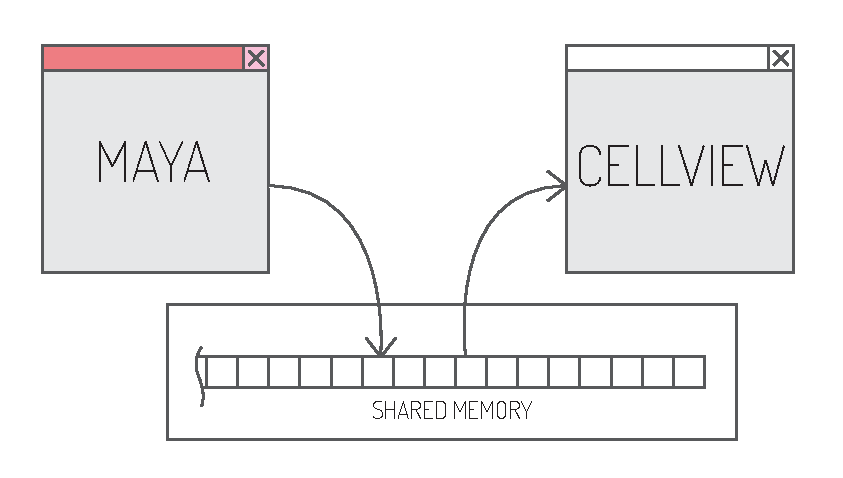
\includegraphics[scale=0.7]{images/method-overview.pdf}
  \caption{High-level overview of the system}
  \label{fig:method-overview}
\end{figure}

%[\textbf{overview of the method: two ends, shared memory, what needs to be transfered, ...}]
On the Figure \ref{fig:method-overview}, you can see an overview of the system. On one side we have a modeling software while on the other we have a domain-specific tool, in our case it is a high performance renderer. Our vision was to have both of these programs running at the same time. The illustrator could have his scene opened in his modeling software. This way he would be using the tools he knows and is accustomed to for modeling the actual scene. Then on the renderer side he would be able to see how the changes he has made are reflected in the rendered final image. This all would happen in real-time thanks to writes and reads into and from shared memory.

% [\textbf{simplifications, how the scene can be described}]
As was already mentioned, when dealing with molecular data we can take advantage of several simplifications. A scene like this consists of macromolecules: proteins and lipids. First simplification—we consider the shape of the molecule to be static. This means that inside each molecule, the positions of all the atoms does not change in time. The position of the atoms is taken from the PDB file. The second simplification is that all the instances of certain molecule type look the same. They only differ in position and rotation.

% [\textbf{what data do we need to transfer}]
With these facts in mind, we can define a molecular scene as a set of molecules, where each molecule is defined by its position, rotation, and type, which says what kind of molecule this instance is.

\begin{figure}
  \centering
  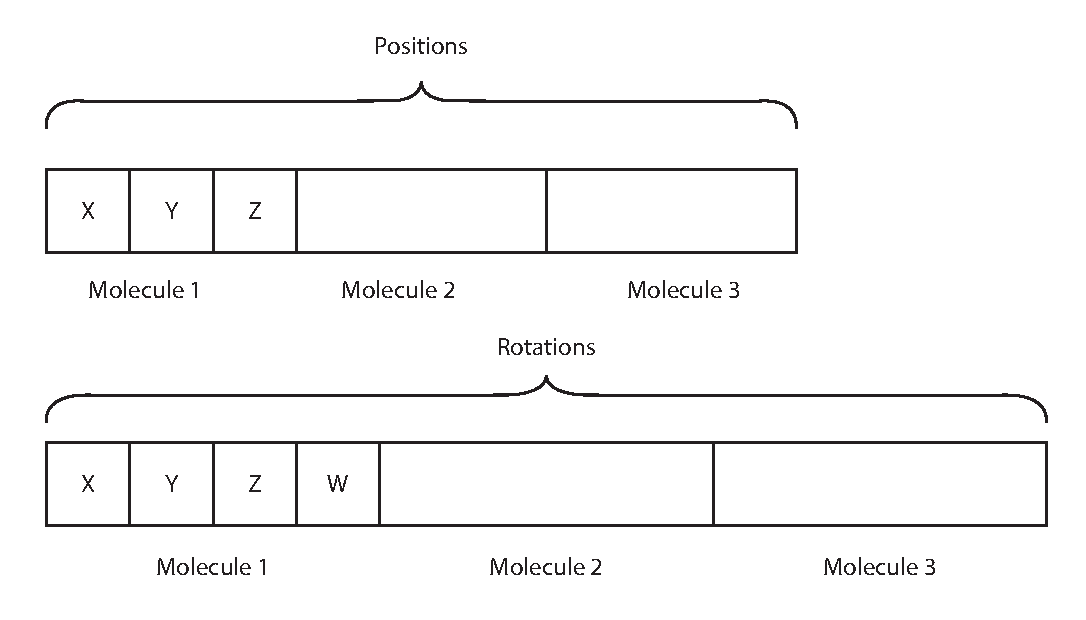
\includegraphics[scale=0.7]{images/data-layout.pdf}
  \caption{Shared memory data layout}
  \label{fig:data-layout}
\end{figure}

This means that we need to stream this data—positions, rotations and types—of all molecule instances from the modeling software to the rendering tool. Because of the technical implications we write the data in a format described on Figure \ref{fig:data-layout}. This is more efficient that writing the data in a format position/rotation/into for each molecule.
\section{Process}
\subsection{Parsing the Scene}
% [\textbf{the actual process}]
Inside the modeling software, we scan the scene, looking for molecular objects. We need to identify an object which is supposed to represent an instance of a molecule. We find out what type of molecule this is. This information is saved in a form of pdb id. For each of the found instances we also read its world position and rotation. This info is accumulated into an array and then prepared to be written into the memory.

There are several approaches and optimizations possible at this level and these depend mostly on the API that the modeling software provides. We were able to inject this method into a callback which is called every time the scene has changed. After this happens, we scan all the models in the scene and look for molecular objects. This could be optimized in a way that only the objects that have changed report their changes. That way not all the object in the scene need to be scanned which saves us some performance. As we have discovered however, the APIs are not always keen on having such a performance-heavy procedures executed on each frame and so the concrete implementation heavily depends on the chosen modeling software and its API. We will describe in more detail how we accomplished this with Maya API in the chapter Implementation.

\subsection{Writing into and Reading from Shared Memory}
Once the data about current state of the scene is accumulated into position, rotation and info arrays, we can write these into the shared memory. Operating system API calls should be used for this. Again, for more details, see chapter Implementation to see how we did this on Windows operating system.

\subsection{Using the data}
Reading the data uses operating system API calls as well. In our case, because we are operating on the interface between c++ and c\#, the code that reads from the memory is pretty simple, only retrieving memory address and sending it into the c\# part of the system. This data is then copied into buffers inside cellVIEW which in turn sends them to GPU for render. We format the data in a way so that there is no additional manipulation on the data between these steps required. After the data write, we ideally want to only copy the chunks of memory from one place to another.

%[\textbf{Why Maya?}]
We have chosen Maya as the modeling software because our collaborating partner, Drew Berry, is its prominent user and he has been a key person that we had in mind when implementing this method. Choosing cellVIEW as the renderer has been an obvious choice as its rendering capabilities are on the state-of-the-art level of what common hardware computers are able to render. Drew Berry has been impressed with the results of cellVIEW and expressed his interest in using it for his movies.

% \section{old}

%[\textbf{we don't want to use files} TODO: why?]Our method tries to solve these two problems. The problem of import/export is solved by using shared memory instead of files managed by the user. The rendering times problem is solved by using modern rendering techniques which enable us to render what we want in an interactive frame-rate.
%The reason why it's possible to take this approach of using shared memory comes from the character of data that we work with. Molecular scenes consist of molecules. Molecules are made of atoms which can be, and usually are, represented as spheres. Atoms of different elements are visualized by having different radii and colors. So for every molecule we need to keep track of what atoms it consists of, positions of those atoms and type of each of those atoms. This is even more leveraged by Protein Data Bank, which stores data about various proteins that have been found through out the years. For us, this means that we only need to keep track of the type of molecule and by fetching data from Protein Data Bank we get information about the protein cataloged under the protein identifier. Our scenes are (simplified) made of macromolecules. That means that in the end for rendering the scene we need a list of molecules, where for each molecule instance we need to save it's position, rotation and type. That's all the info that we need to be able to render our large molecular scenes. Even though this is still a lot of data, we are slowly getting to being able to render this on commonly available hardware. Because of the fact that this data size is "manageable" by modern computers we are able to store the data in shared memory.
%This method is mostly valuable as an example of how interconnection of software can be done and what improvements to the users this can bring. There is some prerequisites - both programs need to be extensible to the extend of the programmers must be able to develop extension that are able to read from and write to the shared memory using operating system API calls.

\chapter{Implementation}
\label{chap:implementation}
This chapter will in detail describe the implementation of real-time scene data sharing between Autodesk Maya and cellVIEW. Autodesk provides Maya users an API which allowed us to extend this program with required functionality. Similarly, we have been able to create plug-in for cellVIEW. This was thanks to the fact that cellVIEW is implemented using Unity engine which also allows custom plug-ins in a form of DLL to be used.

\begin{figure}
  \begin{center}
    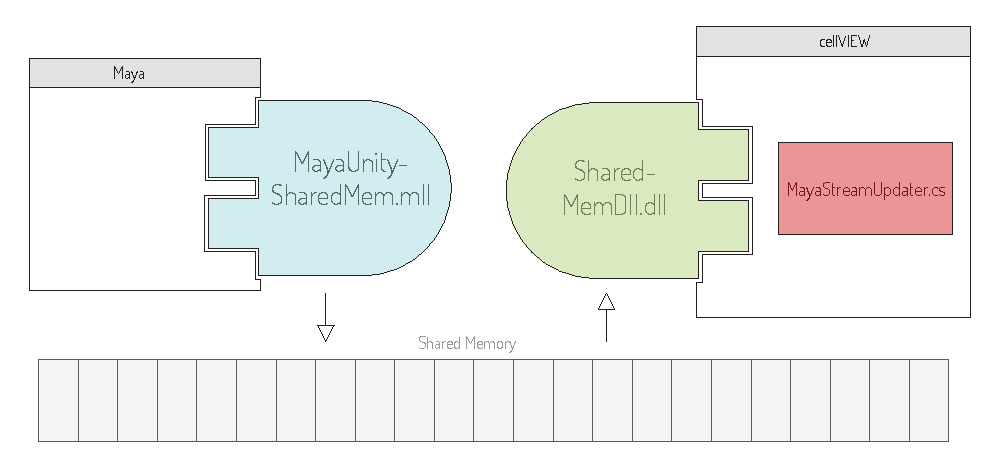
\includegraphics[scale=0.8]{images/system-overview.pdf}
  \end{center}
  \caption{Overview of system components}
  \label{fig:system-overview}
\end{figure}

% [\textbf{high-level overview of the architecture}]
The architecture of the system consists of three parts—a plug-in for Maya, plug-in for Unity and a Unity script—as is shown in Figure \ref{fig:system-overview}.
The data flows only in one way - we write into shared memory with Maya plug-in and read from shared memory with Unity plug-in. This simplifies the situation from the implementation point of view because we do not have to design synchronization scheme.

The plug-in for Maya is using Maya API (which will be described later) and is written in C++ programming language. The function of this plug-in is to parse the 3D scene, looking for a molecular objects, and output their positions and rotations (along with information about the of type of the instance) into the shared memory.

Unity side of the system consists of two parts - a C++ plug-in and a C\# script. The C++ plug-in takes care of reading the data from shared memory, while the C\# script, which is a part of cellVIEW, receives this data and uses them to render the final molecular scene.

Note that there are two types of interoperability between components: (1) shared memory functionality, which enables two processes to communicate, and (2) interoperability between C++ and C\#, which allows us to pass memory addresses from the plug-in to the script on Unity side.

% [\textbf{shared memory} - talk general about shared memory technology]
\section{Shared Memory}
Shared memory is a segment of system memory which can be accessed by multiple programs. It is used as an efficient way to establish communication between separately running processes. Our implementation has been done on Windows, however the concept of shared memory can be found on all operating systems.

% TODO: swaping onto disk, unix, named file mapping in windows
From now on, we will be talking about the implementation that has been done on Windows operating system. There are several ways how we can access shared memory here. boost library provides class that establishes an abstraction above shared memory functionality. Similarly, Qt framework also has class with comparable function set. We chose to not use any of these. Instead, we directly used Windows API function calls to operate with shared memory. This solution has been chosen because we wanted to use the lowest possible layer because of speed concerns. This unfortunately means that our implementation is tied to Windows platform. Porting to other platforms should however be straight-forward either by using operating system specific calls or by using one of the mentioned libraries.

\section{C++ and C\# interoperability}
Unity engine is written with a combination of C++ and C\#/.NET. A .NET API is exposed to users which enables them to write scripts in either C\# or Javascript. These scripts are used to implement gameplay or other behaviour.

\textit{Managed code} is a code which runs under CLR (Common Language Runtime) virtual machine. \textit{Unmanaged code} is any other code which does not need CLR but runs directly on the hardware instead.

C\# and .NET framework have been designed with interoperability in mind. What this means is that programmers can reuse code written in other languages. There are several types of interoperability but we are interested in calling unmanaged (C++) code from a Unity script written in C\#.

We use a feature called Platform Invoke. Platform Invoke enables managed (C\#) code to call unmanaged functions implemented in dynamic link libraries (DLLs).

The process of transforming arguments from types in native code into equivalent types in managed code is called \textit{marshalling}.

%P/Invoke (interoperability of .net code with win32 dlls

% [\textbf{maya api}]
\section{Maya API}

There are two ways how one can extend Maya's functionality—scripts and plug-ins. The technologies which can be used to do so and how they are related is shown in Figure \ref{fig:maya-ecosystem}

Scripting can be done with either MEL or Python and it basically provides an alternative to performing actions via GUI. Everything you can go by clicking in GUI (and sometimes even more) you can do by typing commands through Maya's command line. Longer scripts can be written and run through built-in editor. Scripts are most commonly used for automation.

\begin{figure}
  \centering
  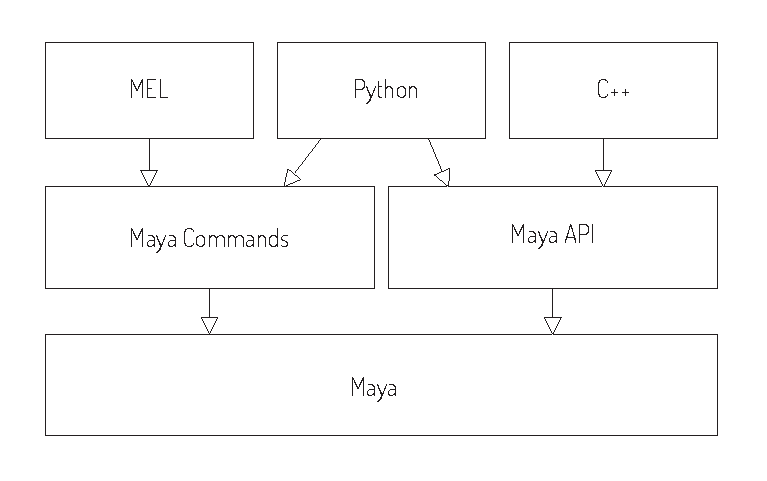
\includegraphics[scale=0.8]{images/maya-ecosystem.pdf}
  \caption{Maya ecosystem}
  \label{fig:maya-ecosystem}
\end{figure}

The second way to extend Maya is by creating plug-ins which use Maya API, either in C++ or Python. There are several types of plug-ins that users can make but typically these are either implementation of new custom MEL command, or implementation of a custom Dependency Graph node type.

It should be noted that both scripts and plug-ins are supposed to work together inside Maya ecosystem. Different means and programming languages should be chosen accordingly to the project. 
%Maya provides two APIs - one in Python \cite{MayaAPIPython} and one in C++ \cite{MayaAPICpp}. In addition to that, there is MEL scripting language \cite{MayaMEL}. Each of these is suitable for different tasks but it should be noted that Maya API and MEL is supposed to work together.

% TODO: talk about plugin types: command, node
% TODo: talk about typlessness

% image: maya pyramid (MEL -> API -> Maya internals

\subsection{MEL vs. Python vs. C++ in Maya}
MEL (Maya Embedded Language) is a scripting similar to other scripting language like Bash or Perl. It is generally the fastest way to customize Maya in any way. For any more complex tasks it is generally better to use Python scripting or even turn the functionality into a plug-in. There is however one task where MEL shines and that is custom GUI building. Even though users can use modified Qt library in their plug-ins, it is way easier to create custom graphics interface with MEL.

Maya API can be thought of as a level directly under MEL scripting. With Maya API, we can create several types of plugin but two most common are new custom command which can then be called with MEL, and a custom Dependency Graph node. Plug-ins using Maya API can be implemented either in Python or C++.

Python is a powerful and easy to learn scripting language. Its advantage is that it is interpreted which means that there is no need for a compilation step. This is beneficial for developers in the phase of prototyping because they can make changes more quickly. The disadvantage is also a consequence of Python being interpreted—Python is expected to be slower than most compiled language like C++. We wanted to implement functionality which works in real-time. For this reason we decided that working in Python was not the ideal approach in this project.

C++ Maya API ended up being what we used to create our custom plug-in. It has been chosen primarily because we wanted to get as much performance as we can. But there is another reason for us to use C++. By doing so we can easily use operating system API to issue function calls that work with shared memory.

\subsection{Dependency Graph}
Maya's internal scene representation is called Dependency Graph. It is a network of nodes where each node has a set of inputs and outputs. Through these inputs and outputs the nodes are connected and data is propagated through the network. The idea is that each node performs some computation using input parameters and forwards the result further. There is an optimization in this approach in that the calculation is only done when the input parameters have changed somehow. If an output of a node is requested when the inputs have not changed, instead of performing the computation, a cached value is returned.

\subsection{DAG Hierarchy}
DAG (Directed Acyclic Graph), as the name suggests, is a structure in which nodes are connected with edges that have an orientation with the constraint that they cannot create loops. In Maya API context this refers to a hierarchy of nodes which establishes parent-child relationships between them.
% TODO: illustrate with transform -> mesh so that I can reference to it in Maya side section

\subsection{Wrappers, Objects, Function Sets and Proxies}
In Maya API, we can find four types of C++ objects: wrappers, objects, function sets and proxies.

\textbf{Wrapper} objects usually provide utility functionality either for easier manipulation with data or mathematics. These include classes like \texttt{MFloatArray}, \texttt{MMatrix}, \texttt{MVector}, \texttt{MQuaternion} or iterators for traversing collectionbs of data - \texttt{MItDependencyGraph}, \texttt{MItMesh}...

\textbf{Objects} and \textbf{Function Sets} are used to access and change internal object in Maya. Objects are instances of class \texttt{MObject} and they basically serve as a handle which only holds the necessary information about kind of object do they point to. In a way Objects are typeless and their type is determined by a mechanism called RTTI (Run Time Type Identification). Function Sets are here to actually perform operations on Objects. Function Set classes always start with a \texttt{MFn*} prefix and they are designed to be compatible with only certain Objects.

\textbf{Proxies} are classes that allow developers to implement new types of objects like custom nodes or commands. Proxy classes are always prefixed with \texttt{MPx*}.

\section{Maya Side}
Multiple approaches how the functionality could be implemented exist. First option is a naive one—in a function which gets called every frame, iterate through all the objects in the scene, identify molecular objects, compile the data into buffers and then write this information into shared memory. Two basic problems have been encountered with this approach. Second implementation attempts to address these issues.

\begin{figure}
  \centering
  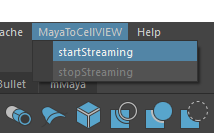
\includegraphics{images/maya-to-unity-menu.png}
  \caption{Maya2CellVIEW menu item}
  \label{fig:maya-menu-item}
\end{figure}

Both of these plug-in implementations have in common that they contain two new custom commands—startStreamingCommand and stopStreamingCommand. When the plug-in is loaded and intialized it creates a new menu item in Maya's main toolbar. Under this menu item there are two sub-items (buttons)—Start Streaming and Stop Streaming (see Figure \ref{fig:maya-menu-item}). These are set up to trigger call of appropriate command—startStreamingCommand and endStreamingCommand. This interface is made to adapt to the state of streaming, you should not be allowed to stop streaming when no streaming is happening and you should not be able to start streaming when you already are.

\subsection{Implementation via Custom Locator}
\begin{figure}
  \centering
  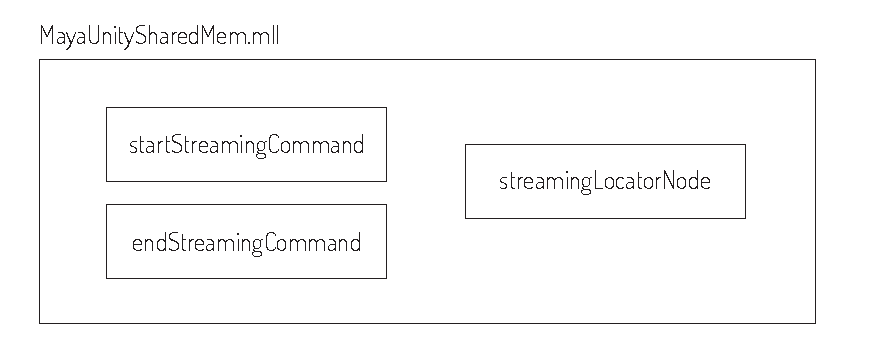
\includegraphics[scale=0.8]{images/plugin-contents.pdf}
  \caption{Plugin contents}
  \label{fig:plugin-content}
\end{figure}
Locator, in Maya API context, is shape that gets drawn but does not show up in the final render. It can serve as a preview of an effect that actually gets rendered but would be too expensive to draw into the interactive viewport. For us, the important fact is that \texttt{MPxLocatorNode} class has a method \texttt{draw}, which gets called everytime something changes in the scene and thus viewport needs to be re-rendered. This is where we can implement our functionality.

This implementation is not exactly in line with Maya philosophy—\texttt{MPxLocatorNode}'s \texttt{draw} method is meant for drawing and not for the type of computation that we need to do there. However, we have tried to implement real-time sharing the way it should be done in Maya—using custom nodes which have input and output attributes and only when the inputs have changed perform the write. Unfortunately this turned out to be performing worse. The rate of change was simply not enough to provide smooth streaming without stuttering.

In the implementation via Custom Locator we do the following. When \texttt{startStreamingCommand} is called, it creates a new instance of the custom locator node and adds it into the scene. From now on, whenever we change something in the scene (move the camera, translate any object, ...) this nodes \texttt{draw} method gets called.

In the \texttt{draw} method, we iterate through all objects in the scene. Looking at the names, we locate either camera or molecular object. Position, rotation and type information is accumulated into three buffers. These are then concatenated and written into the shared memory.

\subsection{Implementation via Watchers}
The previously presented implementation has one disadvantage. Even if just one object changes its position, all the memory is rewritten. Not only that, but we also iterate through the whole scene as well. This could easily become bottleneck. To address this, another approach has been implemented. A concept of a ``watcher'' node has been established.

Upon initialization of the plugin, the whole scene is scanned. When we process a molecular object we create new watcher node. This new node is then connected to the node of a molecular object in a way that the position and rotation attributes are inputs for this watcher node.

Now whenever there is a change in the scene a \texttt{draw} method is called for each instance of watcher node. The position and rotation attributes are read and compared to their previously cached values. If they are the same, nothing gets done. If they are different, we proceed to the memory writing.

Each watcher node knows its index. Using this index the precise address inside the shared memory is computed and we write the new values into the memory at this address.

This approach works better when we are using the plugin for small incremental chances. That is what happens if artist creates the scene, tweaking positions and rotations of individual objects at once. Where this is when the artist makes an animation and plays it back. This way all the watchers write into the memory at the same time. For this use case it would be better if the memory write would be performed only once per frame.
% TODO: mention legacy viewport usage

% TODO: left/right handed conversion
% image: new menu item
\section{Unity side}
%On the side of cellVIEW (or Unity), we have two components - dll plugin and a C\# script.
%Topics - Architecture of the plugin, very generally about plugins (it's just a basic C++ dll plugin), interface between C++ and C\#
cellVIEW has been developed using Unity game engine. Unity allows users to include additional code in the form of two kinds of plugins—Managed plugins and Native plugins.

Managed plugins, similiar to the term managed code, are plugins containing .NET code using CLR virtual machine to execute this code. There is little difference between writting functionality using scripts (common way to code behaviour in Unity) and managed plugins (other than the fact that managed plugins are compiled separately outside of Unity).

Native plugins contain code that is specific to one platform. They allow to call operating system functions or libraries that are not accessible in default Unity.

\subsection{Dynamic-link Library}
SharedMemDll component is a very simple dynamic-link library which encapsulates Windows API function calls. By doing so we can use shared memory functionality in Unity. It consists of two functions—\texttt{get\-Shared\-Memory\-Ptr} and \texttt{cleanup\-Shared\-Memory}.

\texttt{getSharedMemoryPtr} functions opens shared memory segment with a name that is supplied as a parameter to this function. Windows API function \texttt{OpenFileMapping} is used to do that. Then, by calling another WinAPI function \texttt{MapViewOfFile}, we get a pointer to the memory address which we can use to read from this memory. The pointer (of type \texttt{void *}) and a handle (of type \texttt{HANDLE}) are output parameters that are passed on to the C\# script thanks to interoperability feature and marshaling.

\texttt{cleanupSharedMemory} takes care of unmapping a view of file (the pointer) from the process's address space (via \texttt{UnmapViewOfFile}) and closing the handle to the shared memory object (via \texttt{CloseHandle}). Note that shared memory is deallocated when there are no handles attached to this object.

\subsection{Unity Script}
Unity uses scripting as a mechanism for implementing gameplay behaviour. Users can use either C\# or Javascript. The C\# variant is by far the more used one and cellVIEW has also been implemented using C\# scripts.

Every Unity C\# script must be derived from MonoBehaviour class. MonoBehaviour is a base class which implements basic methods like Start, Update, FixedUpdate and OnGUI. Our script, MayaStreamUpdater, is therefore a child class of MonoBehaviour.

We use the two functions implemented in the native DLL plugin by declaring them as private static external methods and using DllImport attribute macro.

In OnEnable method, we call \texttt{getSharedMemoryPtr} to get pointer to shared memory. Four shared memory segments are opened this way:
\begin{itemize}
\item \textit{MayaToUnityPosRotSharedMem}: positions (vector of 4 components), rotations (quaternions) and internal IDs of each protein instance
\item \textit{MayaToUnityCameraInfoSharedMem}: position and rotation of camera
\item \textit{MayaToUnitySceneInfoSharedMem}: general scene information—as of now containing only number of objects in the scene
\item \textit{MayaToUnityPdbMappingSharedMem}: mapping of PDB ID to internal ID.
\end{itemize}

Update method is a MonoBehaviour method that gets called every frame. In Update method of our script, we load the current scene data from shared memory and update the state of cellVIEW so that the updated state gets rendered. First, we load position and rotation of camera and set the current main camera accordingly. [TODO: refine]Unity has the feature that when an attribute of a class which is a child of MonoBehaviour is made public, Unity exposes this property in Unity editor. This way we can declare public \_camera attribute and then assign a Camera object to this attribute from the editor. Position and rotation needs to be transformed because Maya and Unity use different coordinate systems—Maya uses right-handed while Unity uses left-handed coordinate system. Position is transformed easily by inverting the z-coordinate. For transforming the rotation a utility method has been implemented.

Next, positions, rotations and type information is loaded. The layout of this data has been designed with usage in this part of the system in mind. cellVIEW's rendering is based on three buffers - buffer with positions of each instance, buffer with rotations of each instance, and buffer with information about types of each instance. Thus the only action needed is to copy this data from shared memory into these cellVIEW buffers. These are then in turn copied into GPU memory where it is used for actual rendering of the molecular scene.

In current implementation an intermediate step is taken—as in case of camera position and rotation, we need to perform transformation from right-handed (used in Maya) to left-handed (used in Unity) coordinate system. This could be taken care of on Maya side when the data is written into shared memory but because of prototyping reasons this transformation is done in Unity script.

For details about rendering of molecular scenes in cellVIEW please refer to \cite{lemuzic-2014-ivm} and \cite{cellVIEW_2015}.

\chapter{Demonstration}
\label{chap:demonstration}
Here we present two examples of scenes that has been created to showcase abilities of our plugin.

\begin{figure}
  \centering
  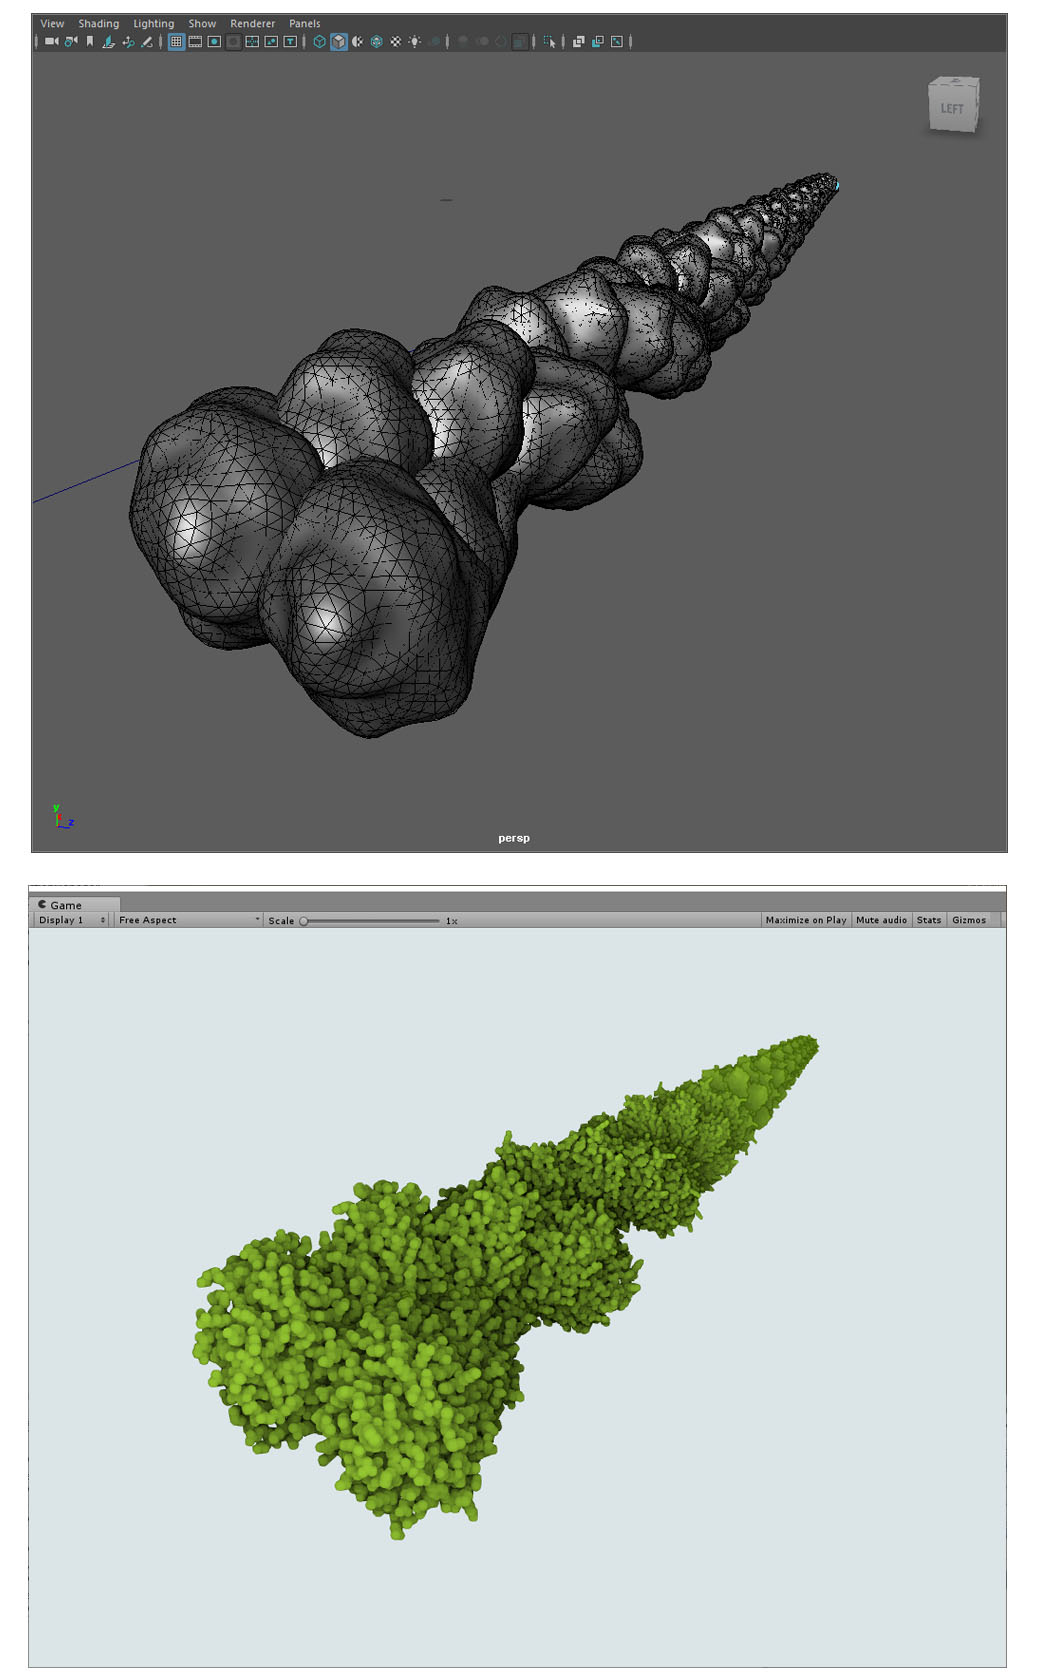
\includegraphics[scale=0.4]{images/strand-1-vertical.jpg}
  \caption{Strand demonstration}
  \label{fig:strand1}
\end{figure}

First use case: strand-like structure displayed on Figure \ref{fig:strand1}. This scene has been created using two additional plug-in: Molecular Maya and Instance around Curve. This is very good because it shows that our plug-in can be used in conjunction with other plug-ins and workflows already existing inside Maya.

Protein has been imported using Molecular Maya. We have downloaded a pdb file from Protein Data Bank and loaded it into Maya with this plugin. Then we exported a low resolution mesh from the protein data. This mesh was then used as an object which was instanced around curve using Instance around Curve plug-in. Last step was to rename the individual instances to a pattern that our plugin would recognise as a molecular object.

%In this chapter we present two use cases of how the user can approach illustration with this new proposed system.
%Use case one - modified Janet's scene.
%Use case two - microtubulus (create a model in maya and then name it properly and we will get it in cellVIEW).

\chapter{Discussion, future work}
\label{chap:discussion}
From the practical point of view, our main goal for this project was to investigate how could we integrate our state-of-the-art renderer cellVIEW into modern professional 3D software.

This has been successfully achieved. Naturally, there is lots to improve upon. Primarily, we would be interested in

Next, working more closely with a scientific illustrator using our system would certainly push this project further.

However, even with this rough prototype we have attracted potentional partners for further cooperation. This project has been presented to Drew Berry who showed his ama. Both side have been eager to , mainly to get some test Maya scenes so that we can try and use it with our system. Unfortunately, we were not able to do this mainly because of other commitments on the side of Drew Berry.

Similar response has been given to Peter Mindek when he presented this project among others from our group and a seminar in Utah. Sweden-dome

Experts from the domain of biology visualization are always eager to tell their stories and express their ideas. It is very common that they want to integrate interactivity in this process. In our other project for example, we developed a demo application which was showing HIV dataset generated with cellPACK. All the proteins have been annotated with a name and a description of its function in this virus. What the experts wanted to create initially was an interactive story—a prepare walkthrough with a commentary about the structure and function of the virus. Unfortunately we have not been able to do this because we did not have proper tools to create this story. Maybe if Maya has been utilized this would have gone the other way. With Maya we could have animated the camera movement on Maya side and then export this movement for replay in cellVIEW.

In this way, we see an incredible potential in this approach. The process of using shared memory for communication between two process has been used in one other project in our group as well. We believe that this could solve a lot of problems in our field. The data that we all try to visualize are mostly the same. There are very few standards so we see that among different programs the data representation stay more or less the same. However as was shown in state of the art, the programs are separated. This leads us to believe that if we can share this (same) data between programs, even better results can be accomplished.

\newpage
\printbibliography[heading=bibintoc]

\appendix %% Start the appendices.
\chapter{Appendix}
%Here you can insert the appendices of your thesis.

\end{document}
